\documentclass[]{ieeeaccess}
\usepackage{cite}
\usepackage{amsmath,amssymb,amsfonts}
\usepackage{algorithmic}
\usepackage{graphicx}
\usepackage{textcomp}
\usepackage{booktabs}
\usepackage{multirow}
\usepackage{siunitx}
\usepackage{subcaption}
\usepackage{hyperref}
\usepackage{color}

\graphicspath{{../results/}}

\begin{document}

\history{Date of publication xxxx 00, 0000, date of current version xxxx 00, 0000.}
\doi{10.1109/ACCESS.2026.0000000}

\title{Bus-Level Inertia Distribution Analysis in IEEE 39-Bus System Under Increasing Renewable Energy Penetration}

\author{
\uppercase{Shakil}\authorrefmark{1},
\uppercase{Ryuto Shigenobu}\authorrefmark{1},
\IEEEmembership{Member, IEEE}
\address[1]{Department of Electrical and Electronic Engineering, University of Fukui, Fukui, Japan}
\tfootnote{Corresponding author: Shakil (e-mail: shakil@example.ac.jp).}
}

\markboth
{Shakil \headeretal: Bus-Level Inertia Distribution Analysis in IEEE 39-Bus System}
{Shakil \headeretal: Bus-Level Inertia Distribution Analysis in IEEE 39-Bus System}

\begin{abstract}
The increasing penetration of inverter-based renewable energy sources (RES) in modern power systems leads to a significant reduction in rotational inertia, thereby threatening frequency stability. Unlike conventional synchronous generators, inverter-based resources (IBRs) inherently provide zero rotational inertia. This paper presents a comprehensive bus-level inertia distribution analysis on the IEEE 39-bus New England system. The proposed methodology utilizes the bus impedance matrix to compute electrical distances between buses and generators, enabling the quantification of effective inertia at each bus location. The aggregated and multi-machine swing equations are employed to simulate frequency dynamics following generator trip events under renewable penetration levels ranging from 0\% to 80\%. Key frequency stability metrics, including the Rate of Change of Frequency (RoCoF) and frequency nadir, are evaluated against grid code thresholds. The results reveal that system inertia decreases by approximately 60\% at 80\% RES penetration, with RoCoF degrading from $-1.13$~Hz/s to $-2.83$~Hz/s. Inertia-weak buses are identified using a spatial distribution index, and the critical penetration threshold beyond which frequency stability limits are violated is determined to be between 60\% and 80\%. The network topology visualization with inertia overlay provides an intuitive spatial understanding of inertia vulnerability across the system.
\end{abstract}

\begin{keywords}
Bus inertia distribution, frequency stability, IEEE 39-bus system, rate of change of frequency (RoCoF), renewable energy penetration, swing equation, system inertia, virtual inertia.
\end{keywords}

\titlepgskip=-15pt

\maketitle

% ============================================================================
\section{Introduction}
\label{sec:introduction}
% ============================================================================

\PARstart{T}{he} global transition toward decarbonized energy systems has accelerated the deployment of renewable energy sources (RES), primarily wind and solar photovoltaic generation. While these inverter-based resources (IBRs) contribute to reducing greenhouse gas emissions, they fundamentally alter the dynamic characteristics of power systems. Unlike conventional synchronous generators, which inherently provide rotational inertia through the kinetic energy stored in their rotating masses, IBRs are connected to the grid via power electronic converters that offer no inherent inertial response~\cite{kundur1994,ulbig2014}.

Rotational inertia is a critical property that determines the initial rate of frequency change following a generation-load imbalance. The system-wide inertia constant $H_{\mathrm{sys}}$ is traditionally computed using the center-of-inertia (COI) formulation as a single scalar value~\cite{kundur1994}. However, as renewable penetration increases and the spatial distribution of synchronous generation becomes non-uniform, treating inertia as a system-wide aggregate becomes insufficient. Recent research has recognized that inertia is spatially distributed across the network, and certain buses may become ``inertia-weak'' due to their electrical remoteness from remaining synchronous generators~\cite{tuo2021,li2024}.

The rate of change of frequency (RoCoF) and frequency nadir are the two primary metrics used to assess frequency stability. Grid codes worldwide impose strict limits on these quantities---typically $\pm 1.0$~Hz/s for RoCoF and a minimum frequency of 59.5~Hz (in 60~Hz systems)~\cite{fernandez2019}. Violations of these thresholds can trigger under-frequency load shedding, generator protection relays, and cascading failures.

Several important contributions have addressed the challenges of low-inertia power systems. Ulbig \textit{et al.}~\cite{ulbig2014} demonstrated the impact of reduced rotational inertia on power system stability and operation. Milano \textit{et al.}~\cite{milano2018} provided a comprehensive survey of the foundations and challenges of low-inertia systems. Bevrani \textit{et al.}~\cite{bevrani2014} surveyed virtual synchronous generator concepts as a countermeasure. Fern\'{a}ndez-Guillam\'{o}n \textit{et al.}~\cite{fernandez2019} reviewed inertia and frequency control strategies, while Dreidy \textit{et al.}~\cite{dreidy2017} classified frequency control techniques for renewable energy sources. More recently, Tuo and Li~\cite{tuo2021} proposed a PMU-based method for dynamic estimation of inertia distribution, and Li \textit{et al.}~\cite{li2024} developed a regional equivalent inertia evaluation method to identify inertia-weak positions.

Despite these advances, a comprehensive study that integrates bus-level inertia distribution analysis with frequency response simulation under progressive renewable penetration scenarios, supported by network topology visualization, remains limited. This paper addresses this gap by presenting a systematic analysis framework applied to the IEEE 39-bus New England system.

The main contributions of this paper are as follows:
\begin{enumerate}
    \item A bus-level inertia distribution methodology based on electrical distance weighting from the bus impedance matrix, enabling the identification of inertia-weak buses.
    \item A comprehensive frequency stability assessment under renewable penetration levels from 0\% to 80\%, quantifying the degradation of RoCoF and frequency nadir.
    \item Multi-machine swing equation simulations revealing the heterogeneous frequency response across generators with different inertia constants.
    \item Network topology visualizations that overlay inertia distribution on the system single-line diagram, providing spatial insight into inertia vulnerability.
\end{enumerate}

The remainder of this paper is organized as follows. Section~\ref{sec:methodology} describes the mathematical formulation and methodology. Section~\ref{sec:system} presents the IEEE 39-bus test system. Section~\ref{sec:results} discusses the simulation results. Section~\ref{sec:conclusion} concludes the paper.

% ============================================================================
\section{Methodology}
\label{sec:methodology}
% ============================================================================

\subsection{System Inertia and the Swing Equation}

The rotational dynamics of synchronous generator $i$ are governed by the swing equation~\cite{kundur1994}:
\begin{equation}
    2 H_i \frac{d\Delta\omega_i}{dt} = P_{m,i} - P_{e,i} - D_i \Delta\omega_i
    \label{eq:swing}
\end{equation}
where $H_i$ is the inertia constant in seconds, $\Delta\omega_i = (\omega_i - \omega_0)/\omega_0$ is the per-unit speed deviation, $P_{m,i}$ and $P_{e,i}$ are the mechanical and electrical power in per unit, and $D_i$ is the damping coefficient.

The system-wide equivalent inertia is defined through the center-of-inertia (COI) formulation:
\begin{equation}
    H_{\mathrm{sys}} = \frac{\displaystyle\sum_{i=1}^{N_g} H_i \cdot S_i}{\displaystyle\sum_{i=1}^{N_g} S_i}
    \label{eq:hsys}
\end{equation}
where $S_i$ is the MVA rating of generator $i$ and $N_g$ is the number of synchronous generators. The total kinetic energy stored in the system is:
\begin{equation}
    E_{\mathrm{kin}} = \sum_{i=1}^{N_g} H_i \cdot S_i \quad [\mathrm{MWs}]
    \label{eq:ekin}
\end{equation}

\subsection{Aggregated Frequency Response Model}

For system-level frequency analysis, the aggregated swing equation with a first-order governor model is employed:
\begin{equation}
    2 H_{\mathrm{sys}} \frac{d\Delta f}{dt} = -\frac{\Delta P}{S_{\mathrm{total}}} - D \cdot \Delta f + P_{\mathrm{gov}}
    \label{eq:agg_swing}
\end{equation}
\begin{equation}
    T_{\mathrm{gov}} \frac{dP_{\mathrm{gov}}}{dt} = -\frac{\Delta f}{R} - P_{\mathrm{gov}}
    \label{eq:governor}
\end{equation}
where $\Delta f$ is the per-unit frequency deviation, $\Delta P$ is the power imbalance in MW, $S_{\mathrm{total}}$ is the total generation capacity in MVA, $D$ is the system damping coefficient, $T_{\mathrm{gov}}$ is the governor time constant, and $R$ is the droop setting.

The analytical expression for the initial RoCoF immediately after a disturbance is:
\begin{equation}
    \mathrm{RoCoF} = \left.\frac{df}{dt}\right|_{t=0^+} = -\frac{\Delta P_{\mathrm{MW}} \cdot f_0}{2 \cdot E_{\mathrm{kin}}}
    \label{eq:rocof}
\end{equation}
where $f_0$ is the nominal frequency. This expression clearly shows the inverse relationship between kinetic energy and the initial rate of frequency decline.

\subsection{Bus-Level Inertia Distribution}

Rather than treating inertia as a system-wide scalar, we compute the effective inertia at each bus using electrical distance weighting~\cite{tuo2021,li2024}. The bus impedance matrix $\mathbf{Z}_{\mathrm{bus}}$ is obtained by inverting the bus admittance matrix:
\begin{equation}
    \mathbf{Z}_{\mathrm{bus}} = \mathbf{Y}_{\mathrm{bus}}^{-1}
    \label{eq:zbus}
\end{equation}

The electrical distance between buses $i$ and $j$ is defined as:
\begin{equation}
    d_{ij} = |Z_{ii} + Z_{jj} - 2Z_{ij}|
    \label{eq:elec_dist}
\end{equation}
where $Z_{ii}$, $Z_{jj}$, and $Z_{ij}$ are elements of $\mathbf{Z}_{\mathrm{bus}}$.

The effective inertia at bus $k$ is computed as a weighted sum of all generator inertia contributions:
\begin{equation}
    H_{\mathrm{eff}}(k) = \frac{\displaystyle\sum_{i=1}^{N_g} w_{ki} \cdot H_i \cdot S_i}{S_{\mathrm{base}}}
    \label{eq:heff}
\end{equation}
where the weights $w_{ki}$ are based on the inverse electrical distance:
\begin{equation}
    w_{ki} = \frac{1/d_{ki}}{\displaystyle\sum_{j=1}^{N_g} 1/d_{kj}}
    \label{eq:weights}
\end{equation}

This formulation captures the physical reality that a generator's inertia contribution to frequency support is stronger at electrically closer buses.

\subsection{Inertia Distribution Index}

To facilitate comparison across different operating conditions, we define the Inertia Distribution Index (IDI) at each bus as the ratio of the local effective inertia to the system-wide equivalent:
\begin{equation}
    \mathrm{IDI}(k) = \frac{H_{\mathrm{eff}}(k)}{H_{\mathrm{sys}}}
    \label{eq:idi}
\end{equation}

Buses with $\mathrm{IDI} < 1$ receive less inertia support than the system average and are classified as inertia-weak.

\subsection{Renewable Penetration Modeling}

Renewable penetration is modeled by progressively replacing synchronous generators with IBRs that contribute zero rotational inertia ($H = 0$). The replacement order prioritizes generators with the smallest inertia constant first, reflecting the practical tendency to retire less efficient, older units~\cite{ulbig2014}. At each penetration level, the modified system inertia becomes:
\begin{equation}
    H_{\mathrm{sys}}^{\prime} = \frac{\displaystyle\sum_{i \in \mathcal{G}_{\mathrm{sync}}} H_i \cdot S_i}{\displaystyle\sum_{i=1}^{N_g} S_i}
    \label{eq:hsys_mod}
\end{equation}
where $\mathcal{G}_{\mathrm{sync}}$ denotes the set of remaining synchronous generators.

% ============================================================================
\section{Test System}
\label{sec:system}
% ============================================================================

The IEEE 39-bus New England system~\cite{kundur1994} is adopted as the test system. It comprises 39 buses, 10 synchronous generators, 35 transmission lines, 11 transformers, and 21 loads. The total generation capacity is 7{,}700~MVA. Table~\ref{tab:gen_data} summarizes the generator parameters.

\begin{table}[!t]
\centering
\caption{IEEE 39-Bus System Generator Parameters}
\label{tab:gen_data}
\begin{tabular}{ccccr}
\toprule
Bus & Gen. & $H$ (s) & $S$ (MVA) & $E_{\mathrm{kin}}$ (MWs) \\
\midrule
30 & G1  & 4.20 & 350  & 1{,}470 \\
31 & G2  & 3.03 & 830  & 2{,}515 \\
32 & G3  & 3.58 & 620  & 2{,}220 \\
33 & G4  & 2.86 & 750  & 2{,}145 \\
34 & G5  & 2.60 & 560  & 1{,}456 \\
35 & G6  & 3.48 & 680  & 2{,}366 \\
36 & G7  & 2.64 & 580  & 1{,}531 \\
37 & G8  & 2.43 & 890  & 2{,}163 \\
38 & G9  & 3.45 & 1{,}040 & 3{,}588 \\
39 & G10 & 5.00 & 1{,}400 & 7{,}000 \\
\midrule
\multicolumn{2}{c}{Total} & $H_{\mathrm{sys}}=3.436$ & 7{,}700 & 26{,}454 \\
\bottomrule
\end{tabular}
\end{table}

The simulation parameters are: nominal frequency $f_0 = 60$~Hz, damping coefficient $D = 2.0$~pu, governor time constant $T_{\mathrm{gov}} = 0.2$~s, and droop $R = 0.05$~pu. The RoCoF limit is set at 1.0~Hz/s and the frequency nadir limit at 59.5~Hz, consistent with typical North American grid codes.

The generator replacement order for renewable penetration studies is G8, G5, G7, G4, G2, G3, G1, G6, G9, G10 (ascending order of inertia constant $H$).

% ============================================================================
\section{Results and Discussion}
\label{sec:results}
% ============================================================================

\subsection{Base Case Inertia Distribution}

Fig.~\ref{fig:topology_base} shows the IEEE 39-bus network topology with bus nodes colored according to their effective inertia $H_{\mathrm{eff}}$. Generator buses are represented as squares, and load/tie buses as circles. The color scale ranges from red (low inertia) to green (high inertia).

\begin{figure}[!t]
\centering
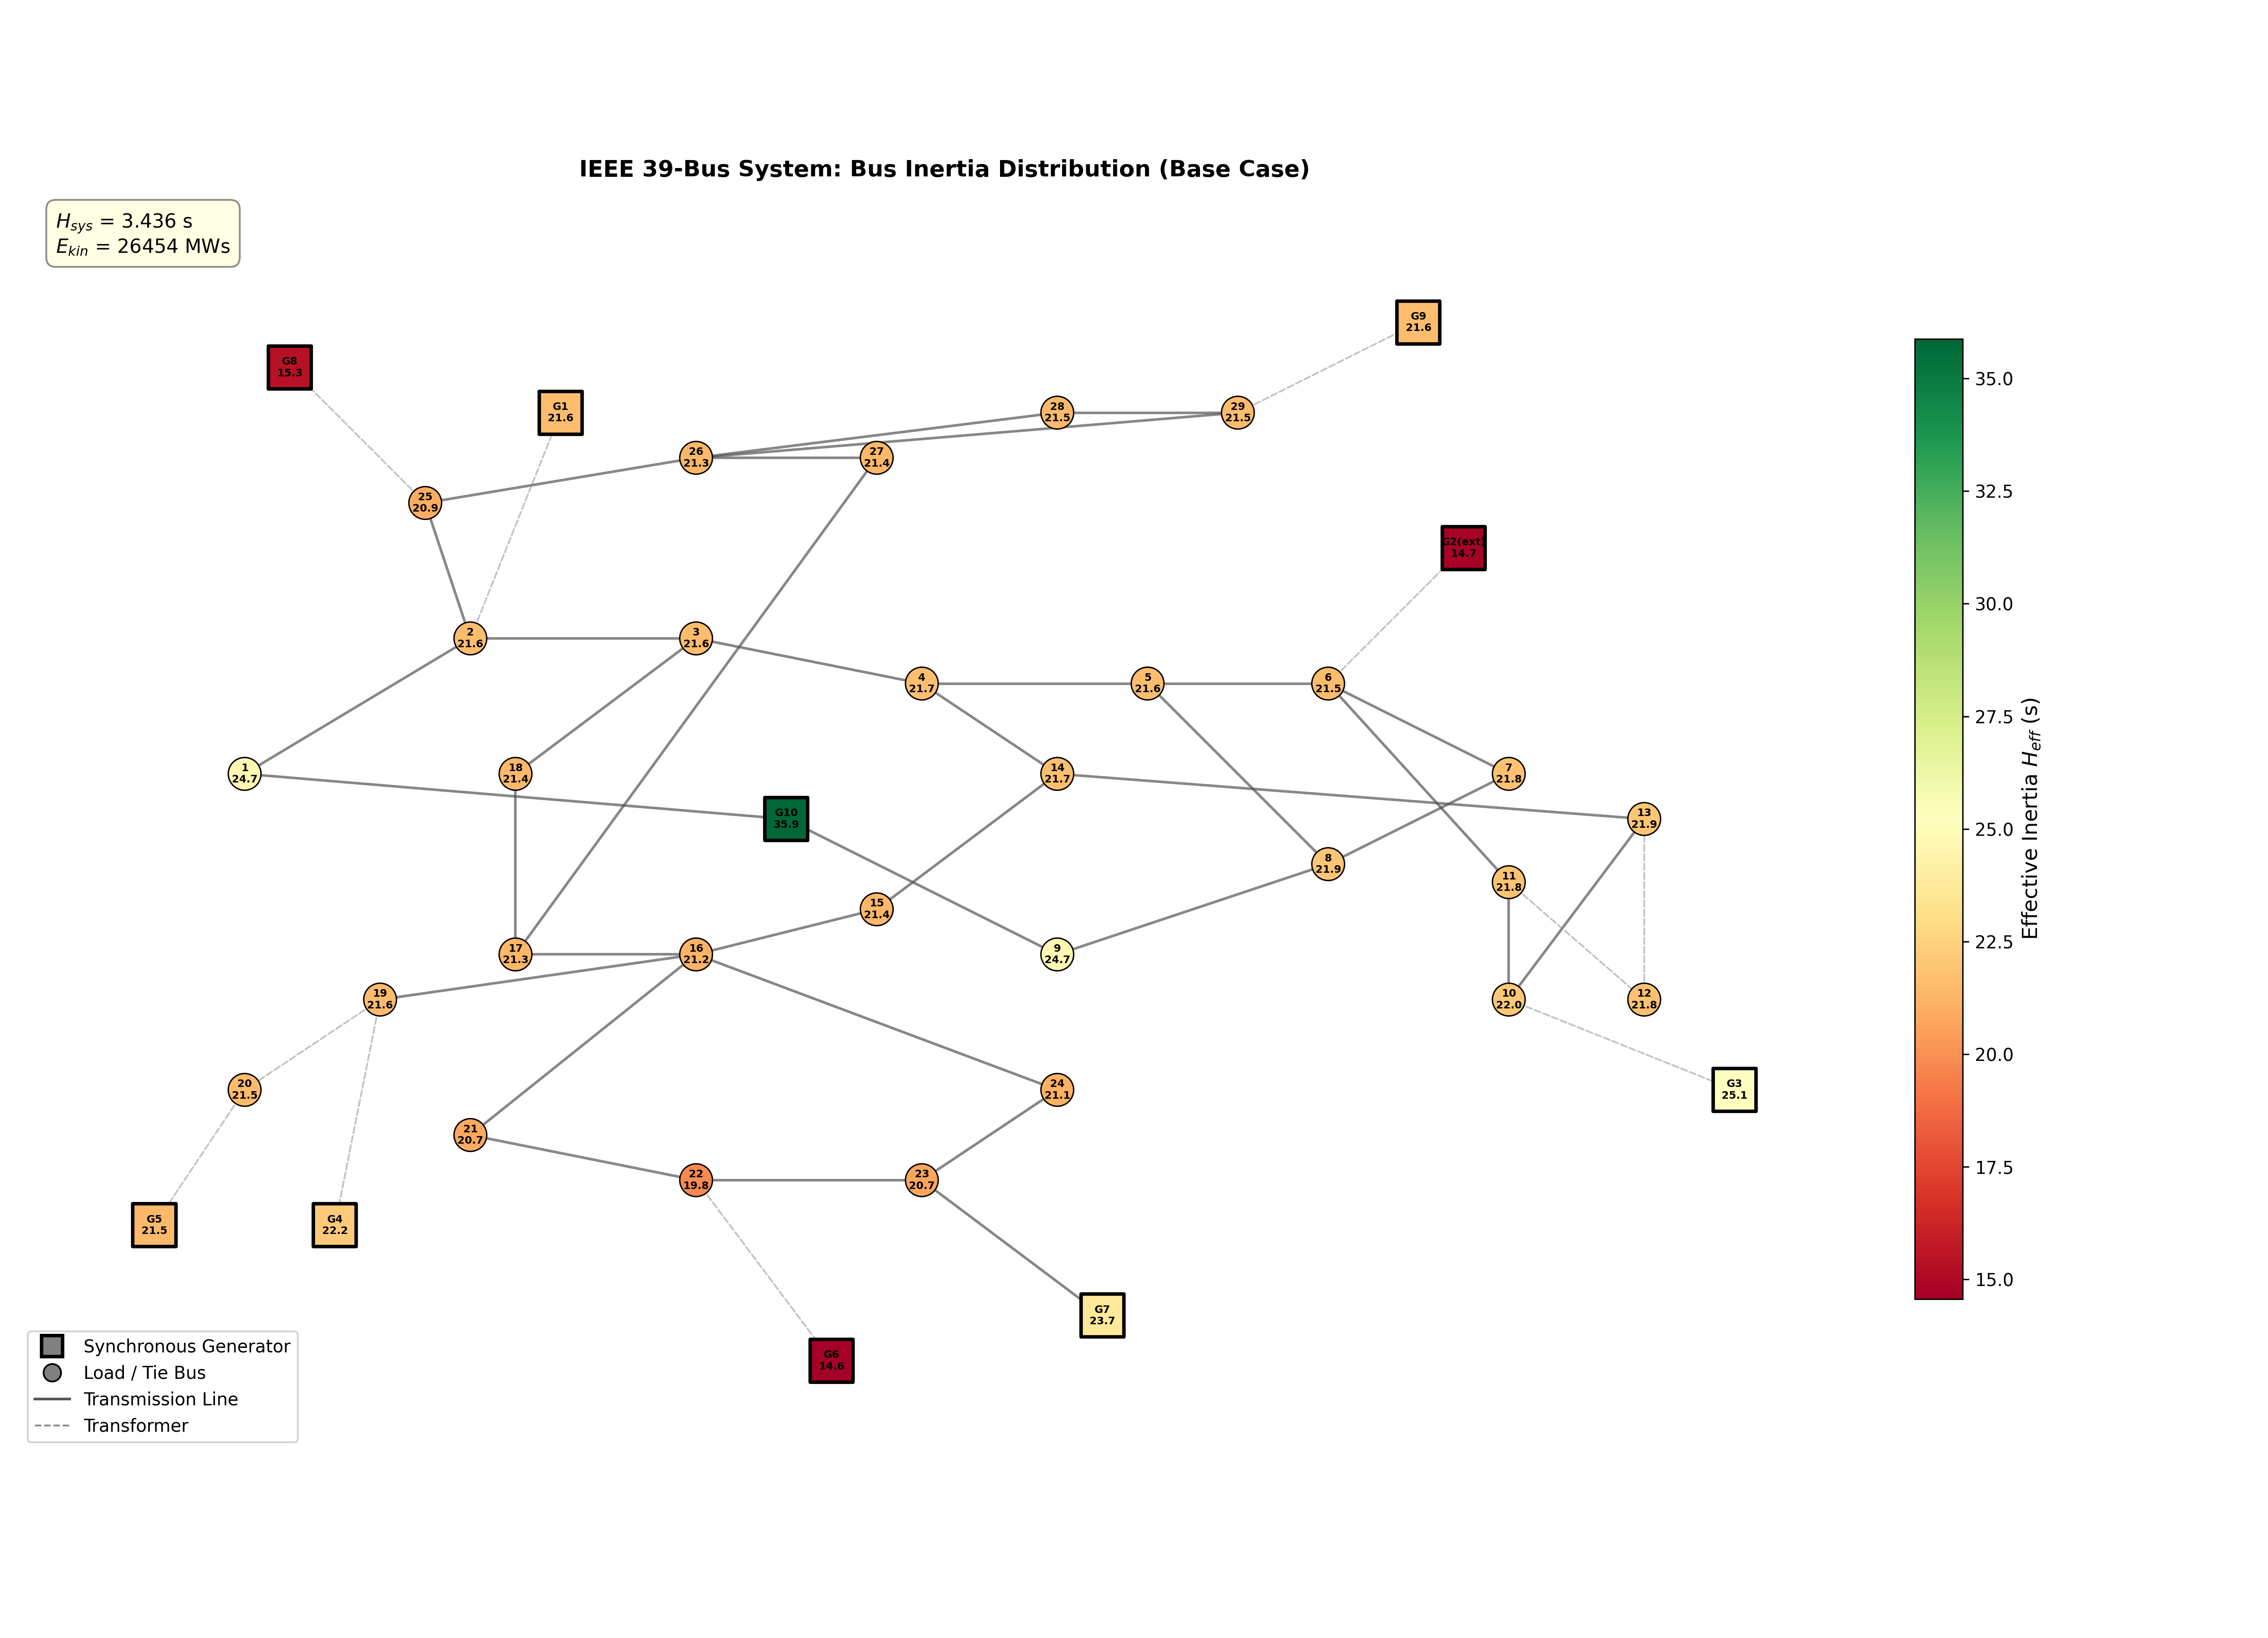
\includegraphics[width=\columnwidth]{fig7_topology_base.png}
\caption{IEEE 39-bus system topology with bus inertia distribution overlay (base case). Squares represent generator buses; circles represent load/tie buses. Color indicates effective inertia $H_{\mathrm{eff}}$.}
\label{fig:topology_base}
\end{figure}

The bus inertia distribution reveals significant spatial heterogeneity. Fig.~\ref{fig:bar_inertia} presents a bar chart of $H_{\mathrm{eff}}$ at each bus. Bus~38 (near G9, rated at 1{,}040~MVA) exhibits the highest effective inertia of 35.88~s, while Bus~34 (G5, rated at 560~MVA) has the lowest at 14.56~s. This 2.5:1 ratio demonstrates that inertia support is far from uniform across the network.

\begin{figure}[!t]
\centering
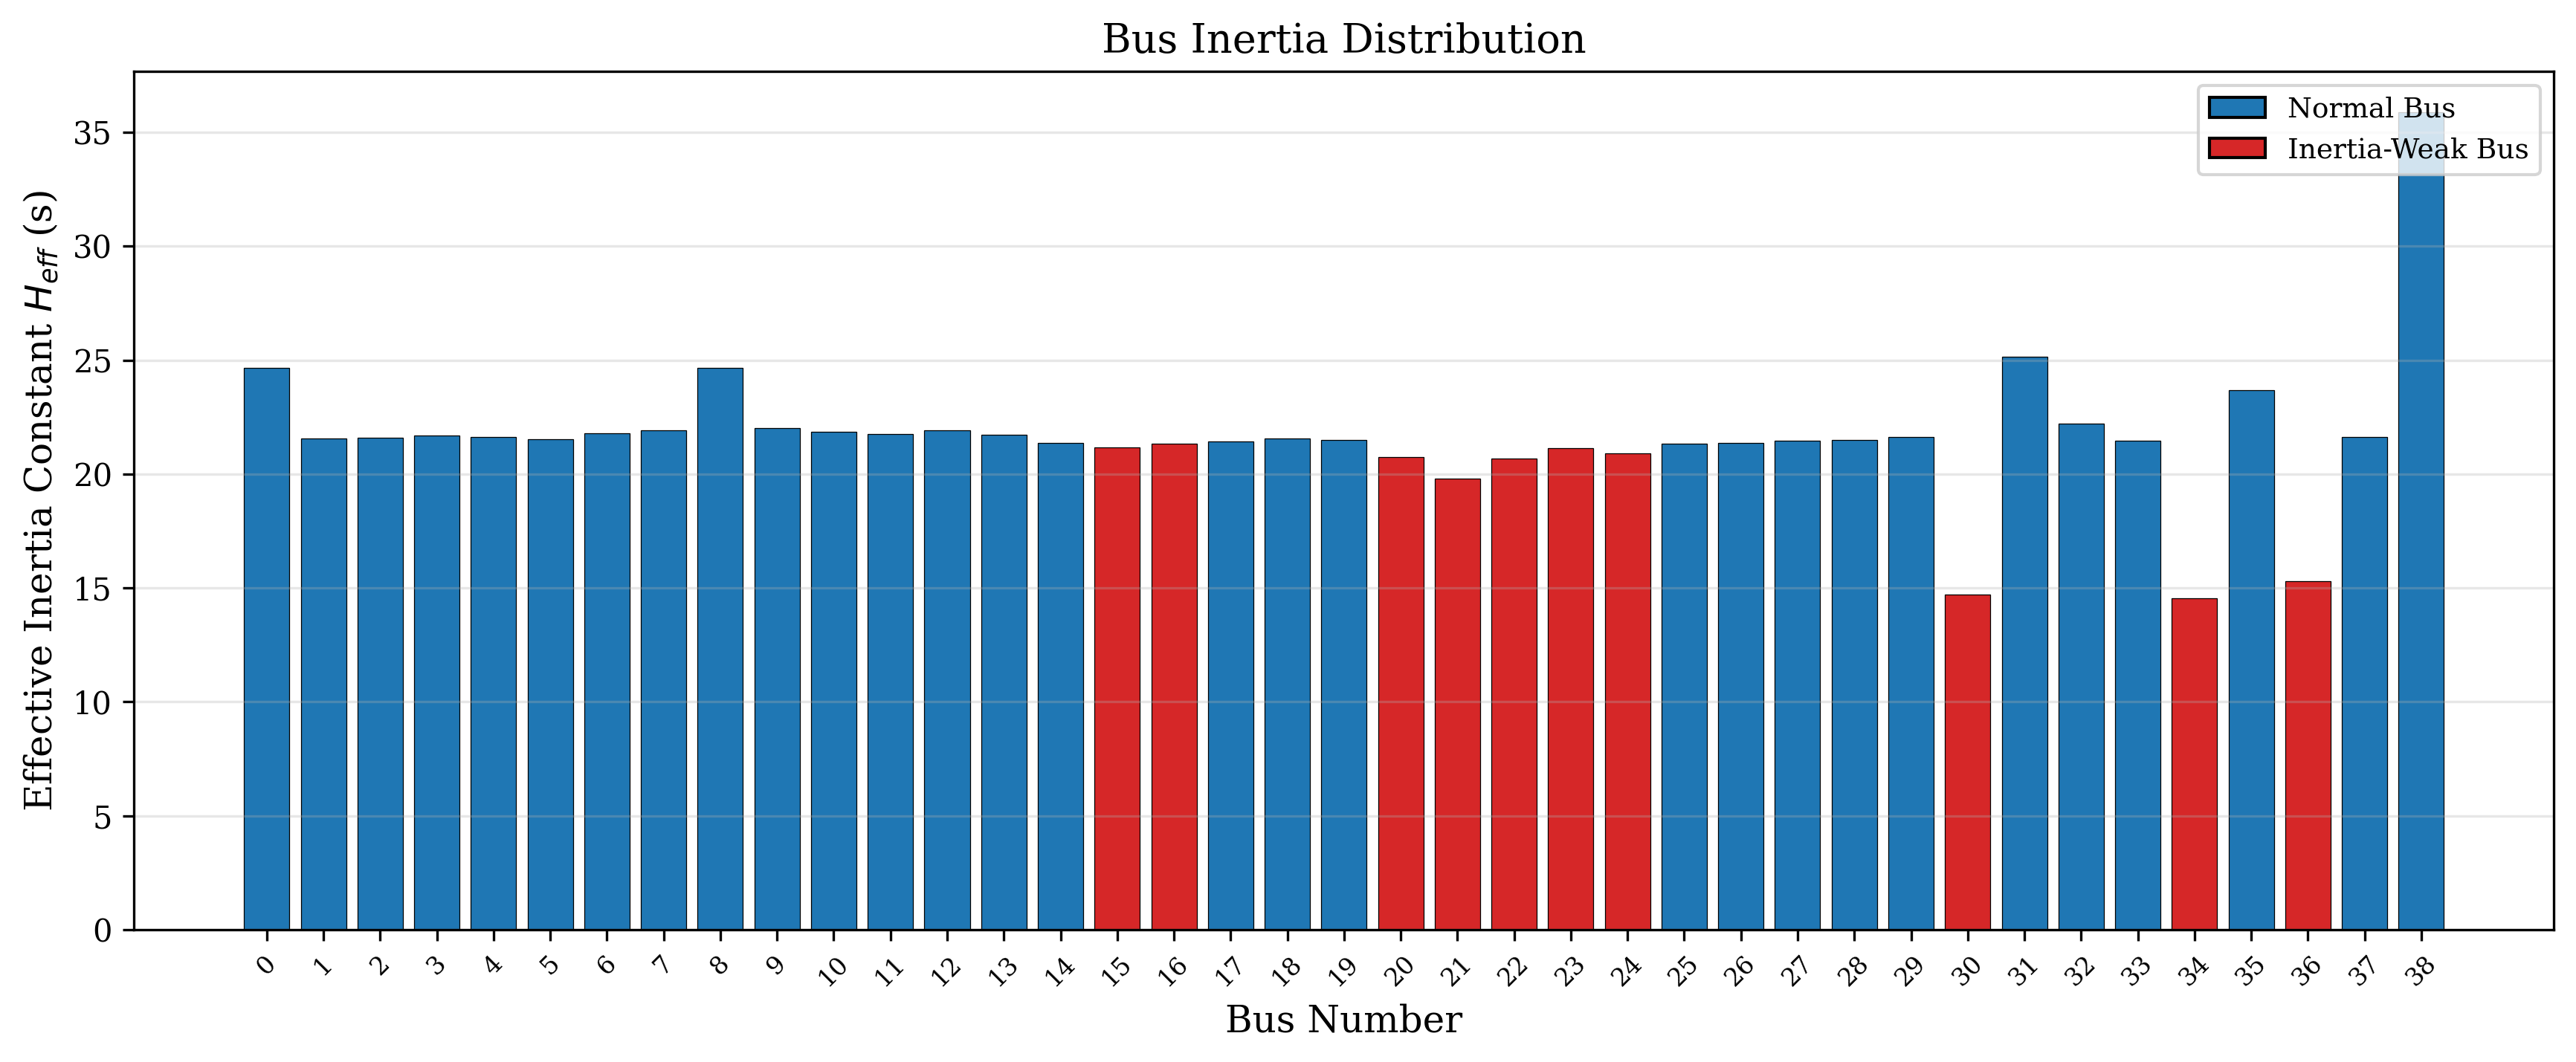
\includegraphics[width=\columnwidth]{fig1_bus_inertia_distribution.png}
\caption{Effective inertia constant $H_{\mathrm{eff}}$ at each bus (base case). Red bars indicate inertia-weak buses (bottom 25th percentile).}
\label{fig:bar_inertia}
\end{figure}

Ten buses are identified as inertia-weak (below the 25th percentile): Buses~34, 30, 36, 21, 22, 20, 24, 23, 15, and~16. Fig.~\ref{fig:topology_weak} highlights these weak buses with red circles on the network topology. Notably, the inertia-weak buses cluster in two regions: (1)~the southern part of the network around Buses~20--24, which are electrically distant from the large generators G9 and G10, and (2)~the generator buses with small-rated machines (G1, G5, G7).

\begin{figure}[!t]
\centering
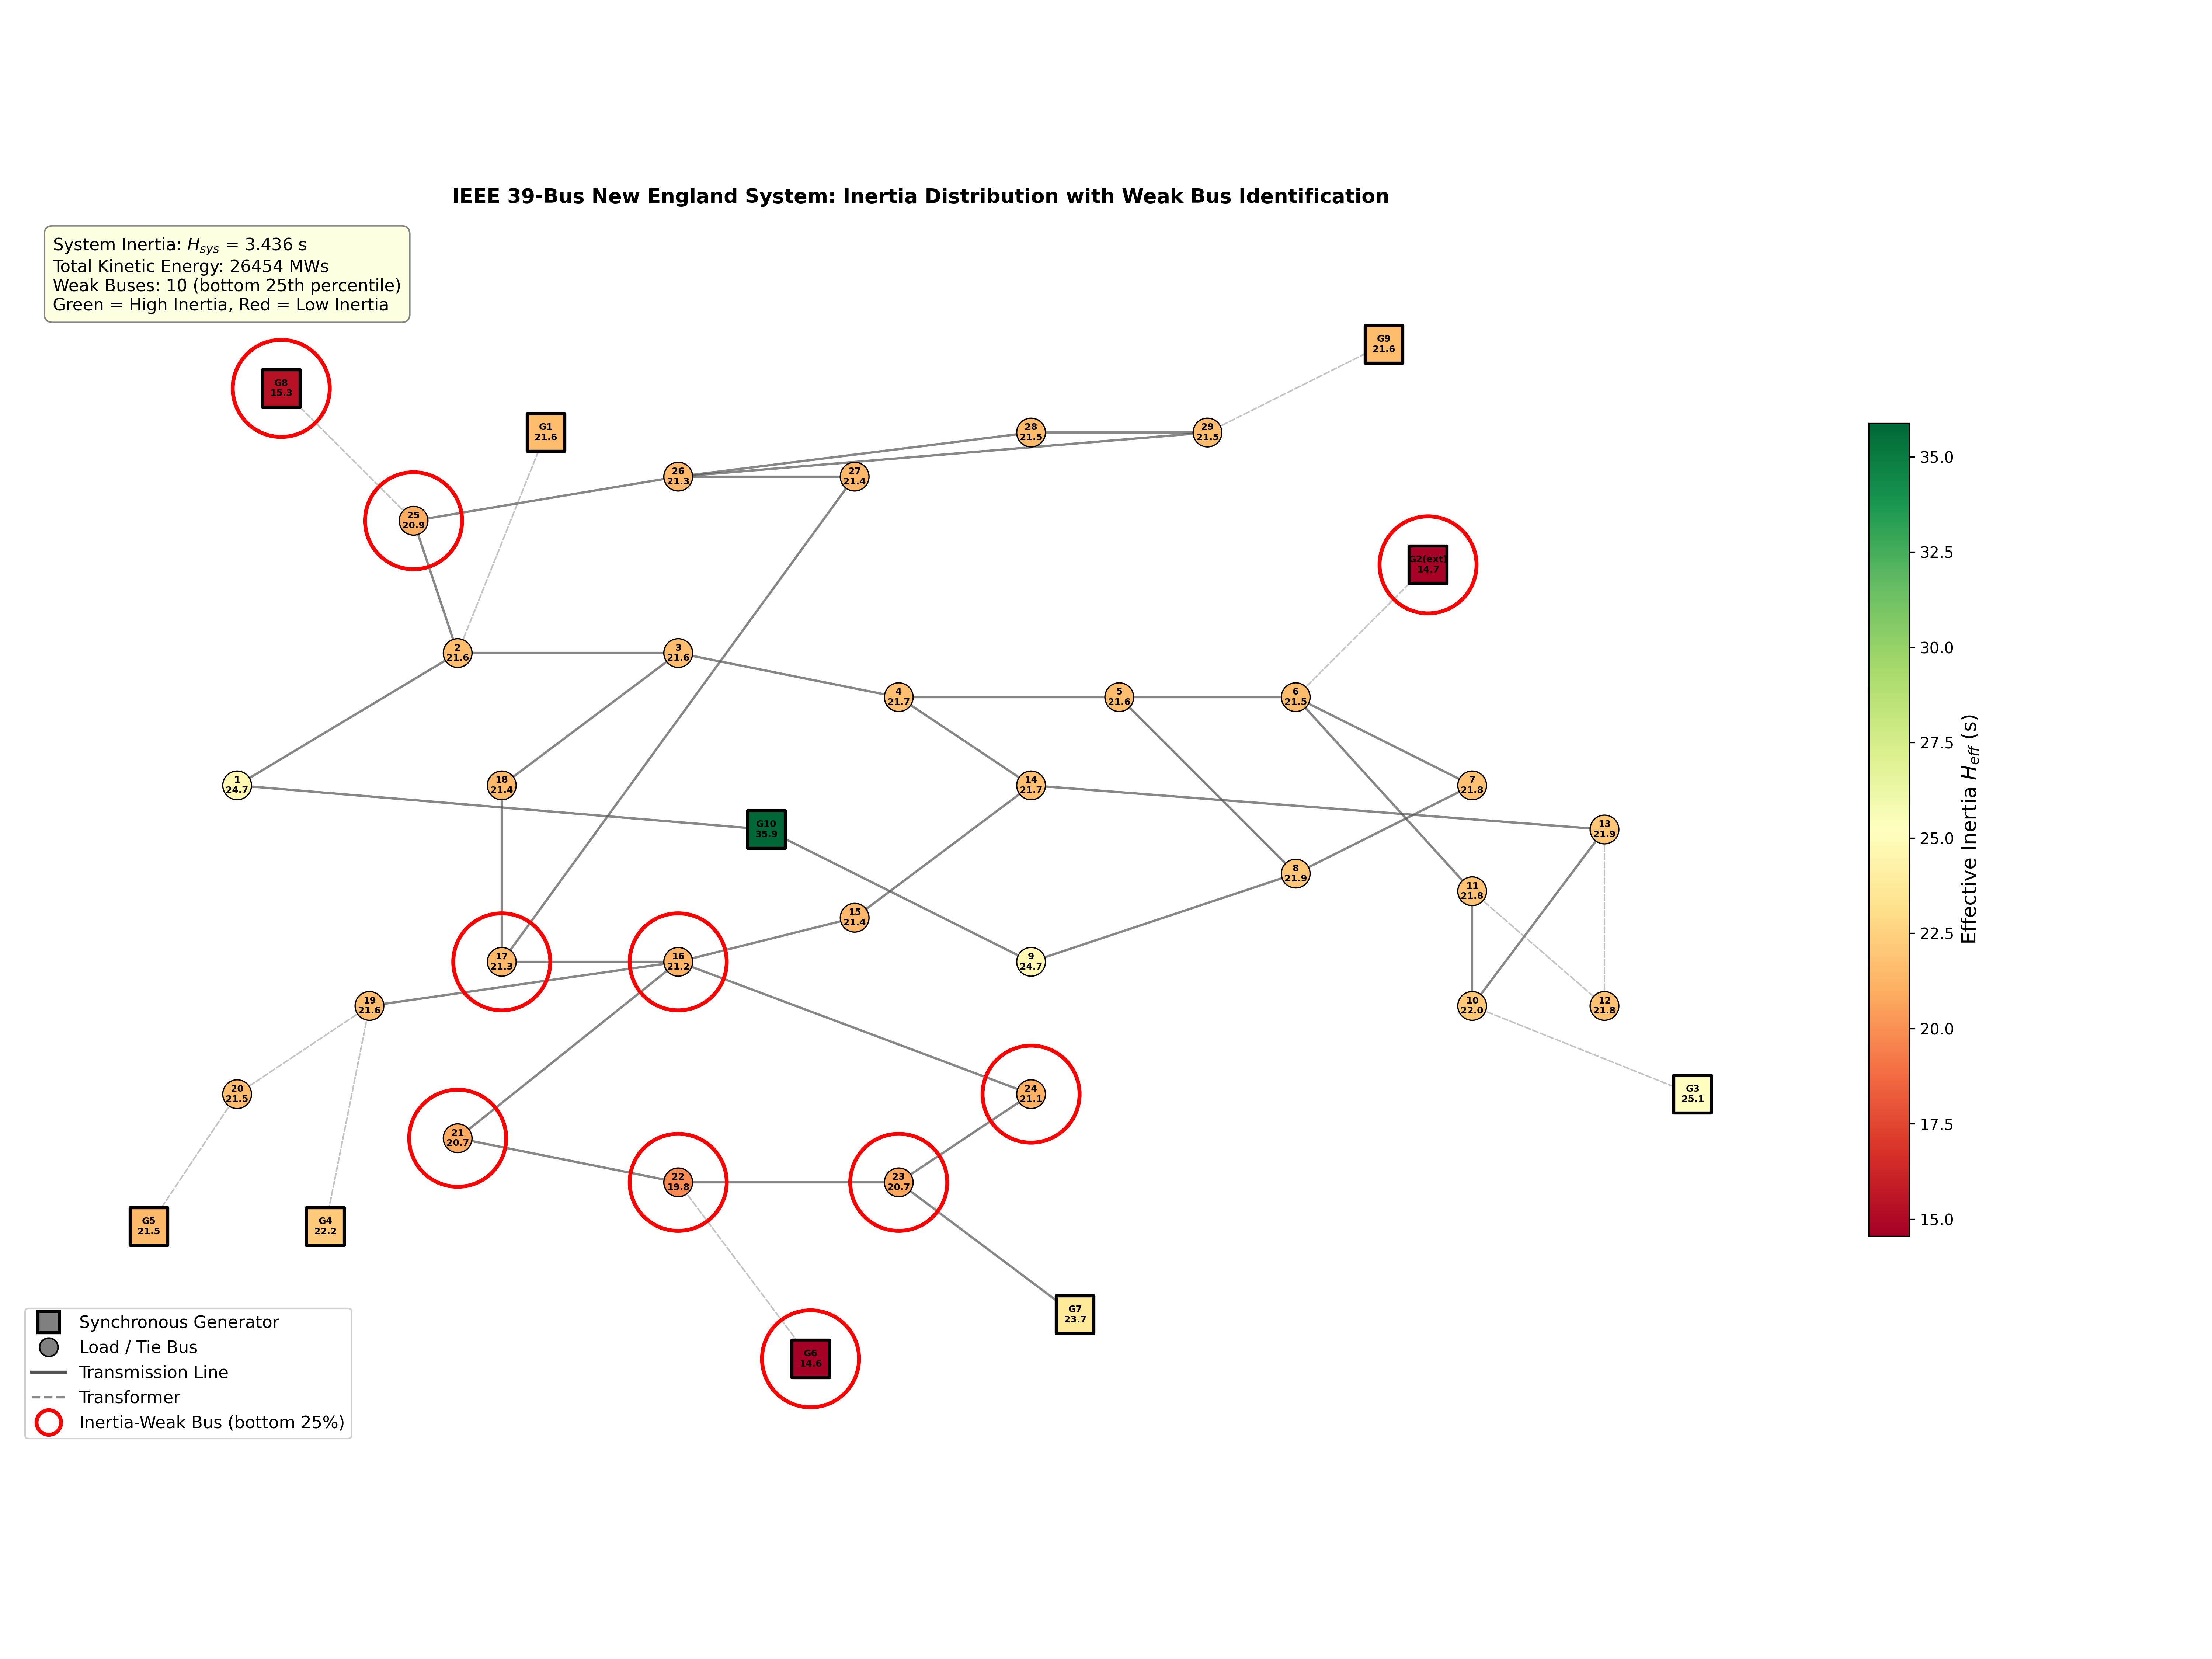
\includegraphics[width=\columnwidth]{fig9_topology_annotated.png}
\caption{Inertia-weak bus identification on the network topology. Red circles highlight buses in the bottom 25th percentile of effective inertia.}
\label{fig:topology_weak}
\end{figure}

\subsection{Frequency Response After Generator Trip}

Three generator trip scenarios are simulated using the aggregated swing equation model~(\ref{eq:agg_swing})--(\ref{eq:governor}). Table~\ref{tab:trip_results} summarizes the results.

\begin{table}[!t]
\centering
\caption{Frequency Response Metrics for Generator Trip Scenarios}
\label{tab:trip_results}
\begin{tabular}{lccccc}
\toprule
Scenario & $\Delta P$ & RoCoF & Nadir & RoCoF & Nadir \\
         & (MW)       & (Hz/s) & (Hz)  & OK?   & OK? \\
\midrule
Trip G8  & 540   & $-0.612$ & 59.788 & \checkmark & \checkmark \\
Trip G10 & 1{,}000 & $-1.134$ & 59.608 & $\times$   & \checkmark \\
Trip G2  & 573   & $-0.650$ & 59.776 & \checkmark & \checkmark \\
\bottomrule
\end{tabular}
\end{table}

The trip of the largest generator G10 (1{,}000~MW) produces an initial RoCoF of $-1.134$~Hz/s, exceeding the 1.0~Hz/s grid code limit. The analytical RoCoF from~(\ref{eq:rocof}) and the simulated value agree within 0.2\%, validating the simulation approach. Fig.~\ref{fig:freq_response} shows the frequency trajectory for the G10 trip scenario, illustrating the frequency nadir of 59.608~Hz at $t = 1.745$~s followed by recovery through governor action.

\begin{figure}[!t]
\centering
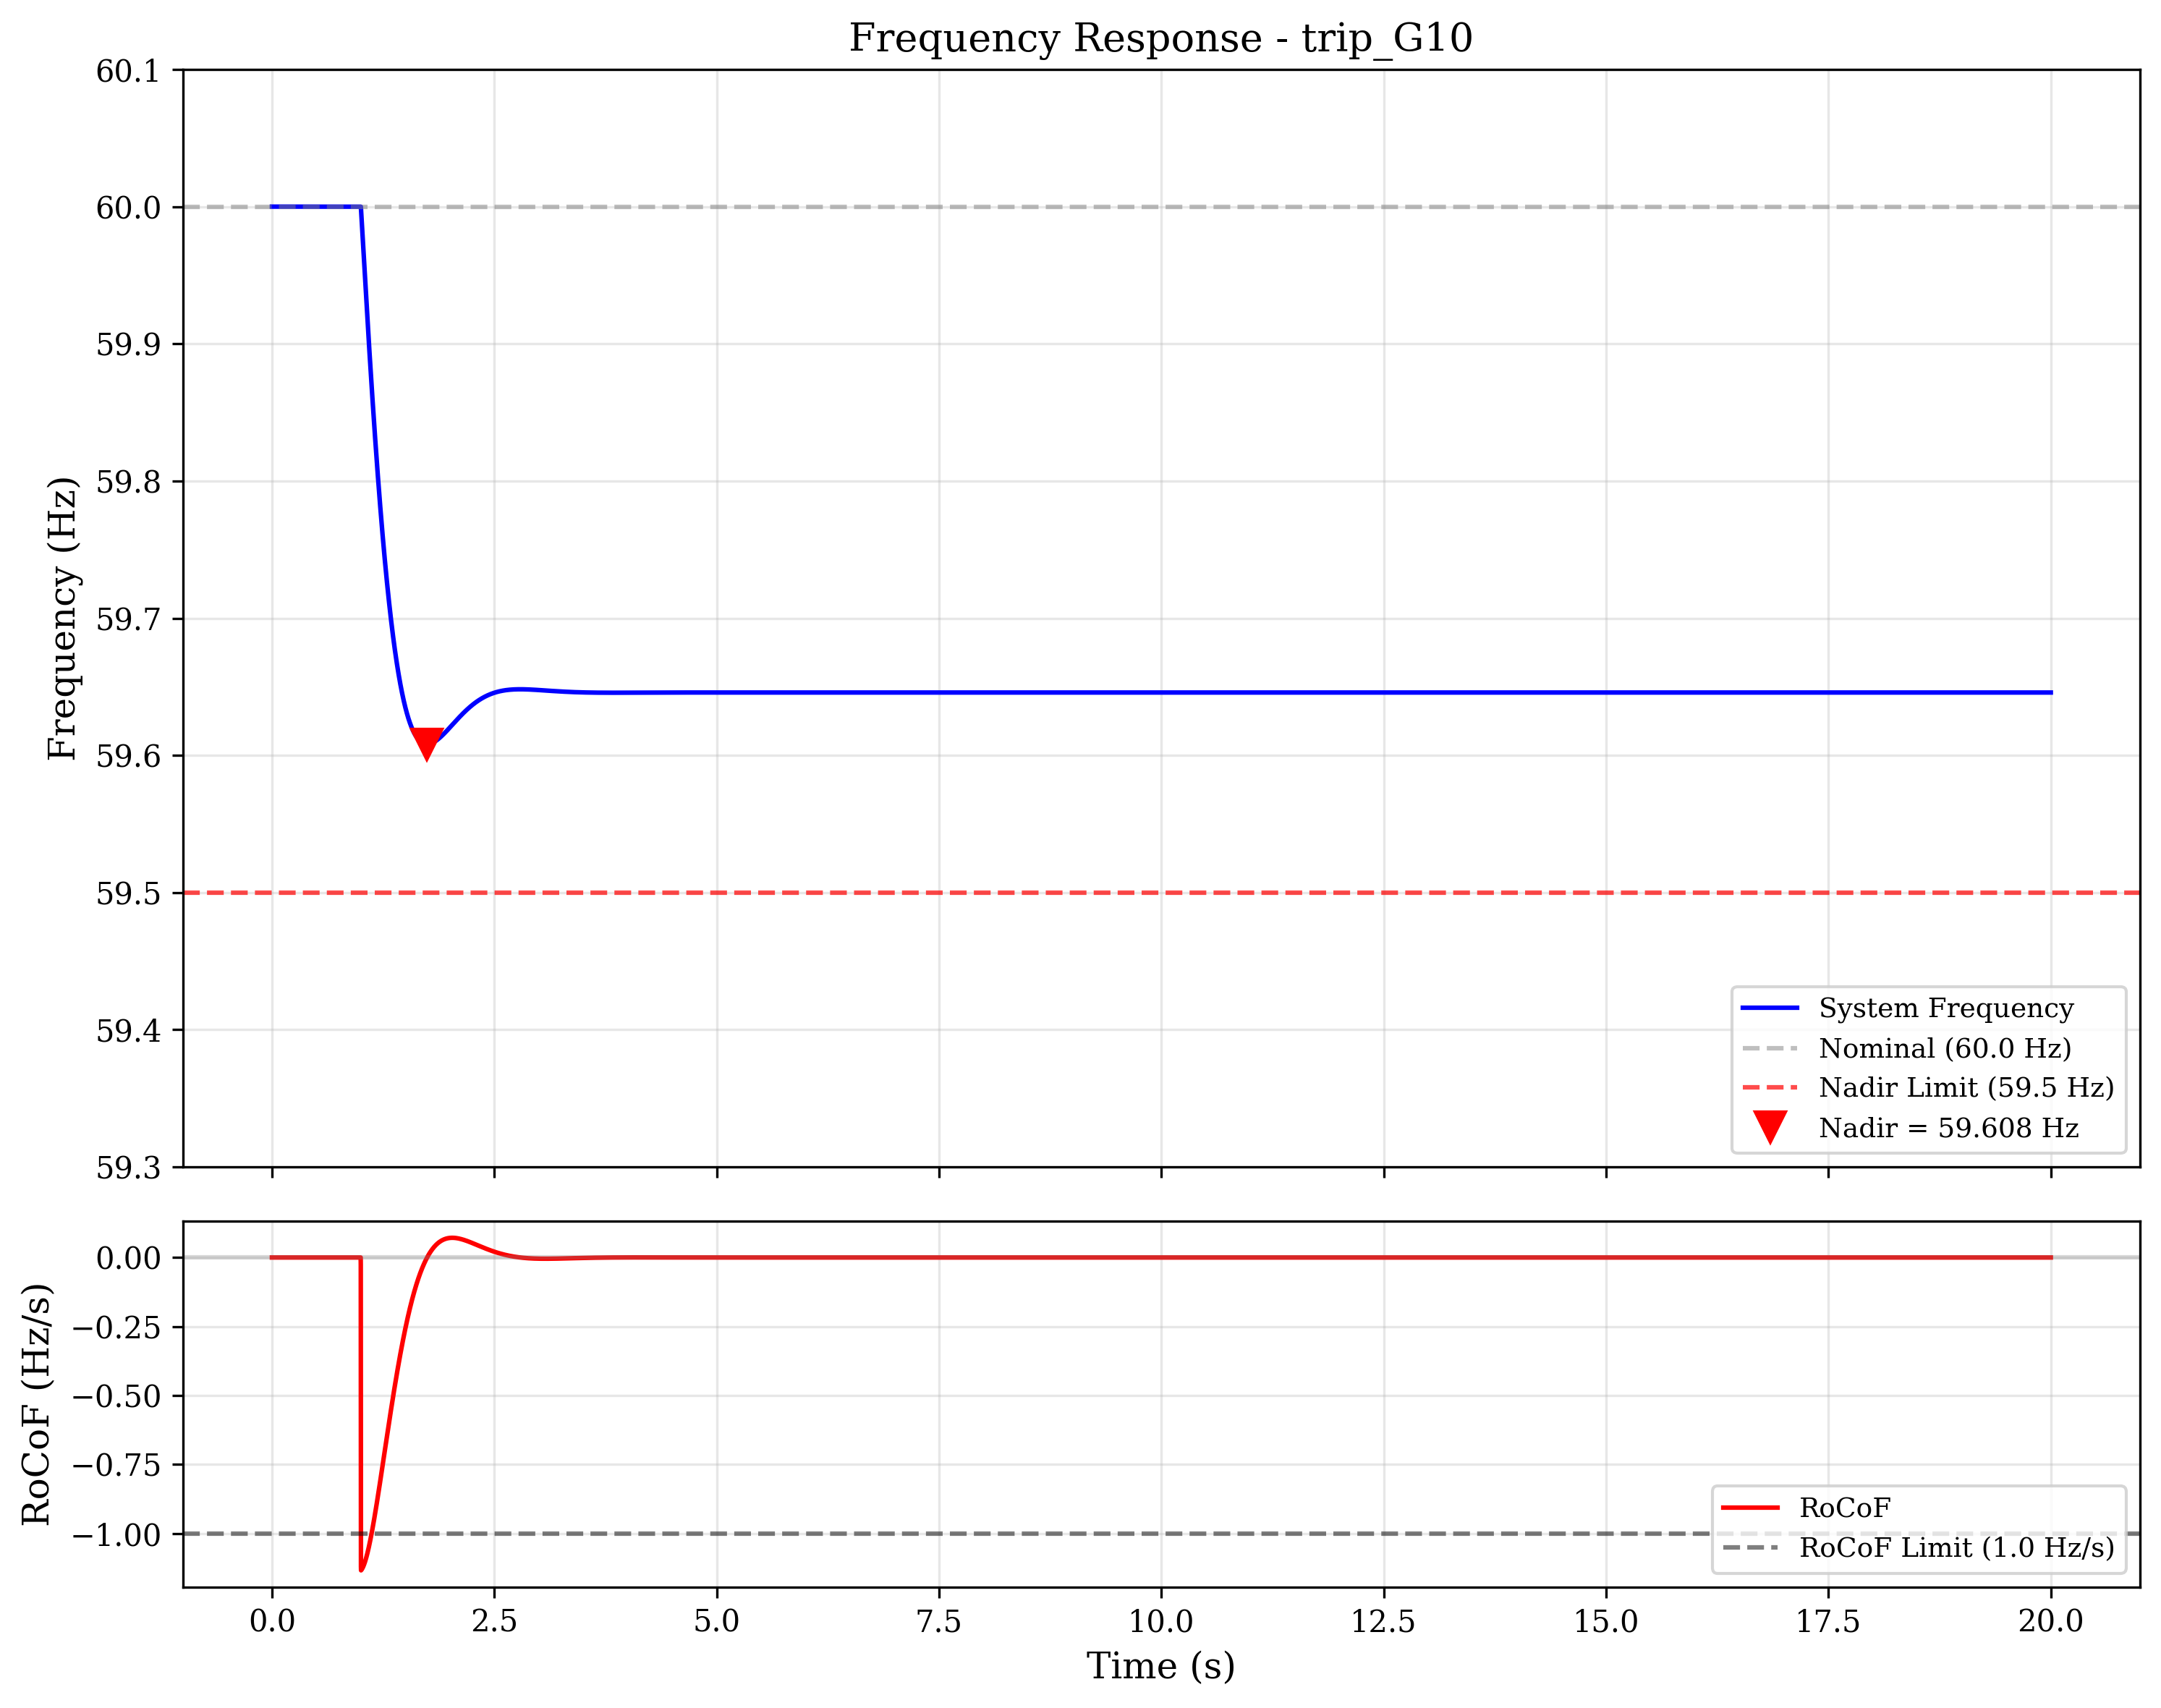
\includegraphics[width=\columnwidth]{fig2_trip_G10.png}
\caption{System frequency response after G10 trip (1{,}000~MW loss). Top: frequency trajectory with nadir marked. Bottom: RoCoF with threshold line.}
\label{fig:freq_response}
\end{figure}

\subsection{Impact of Renewable Penetration}

Fig.~\ref{fig:penetration} presents the degradation of frequency stability metrics as renewable penetration increases from 0\% to 80\%. Table~\ref{tab:penetration} provides detailed numerical results.

\begin{table}[!t]
\centering
\caption{Impact of Renewable Penetration on Frequency Stability (G10 Trip, 1{,}000~MW)}
\label{tab:penetration}
\begin{tabular}{ccrccl}
\toprule
RES & $H_{\mathrm{sys}}$ & $E_{\mathrm{kin}}$ & RoCoF & Nadir & Replaced \\
(\%) & (s) & (MWs) & (Hz/s) & (Hz) & Generators \\
\midrule
0  & 3.436 & 26{,}454 & $-1.134$ & 59.608 & --- \\
20 & 2.966 & 22{,}835 & $-1.314$ & 59.594 & G8, G5 \\
40 & 2.488 & 19{,}159 & $-1.566$ & 59.574 & +G7, G4 \\
60 & 1.682 & 12{,}954 & $-2.316$ & 59.519 & +G2, G3, G1 \\
\textbf{80} & \textbf{1.375} & \textbf{10{,}588} & $\mathbf{-2.833}$ & \textbf{59.486} & +G6 \\
\bottomrule
\end{tabular}
\end{table}

\begin{figure}[!t]
\centering
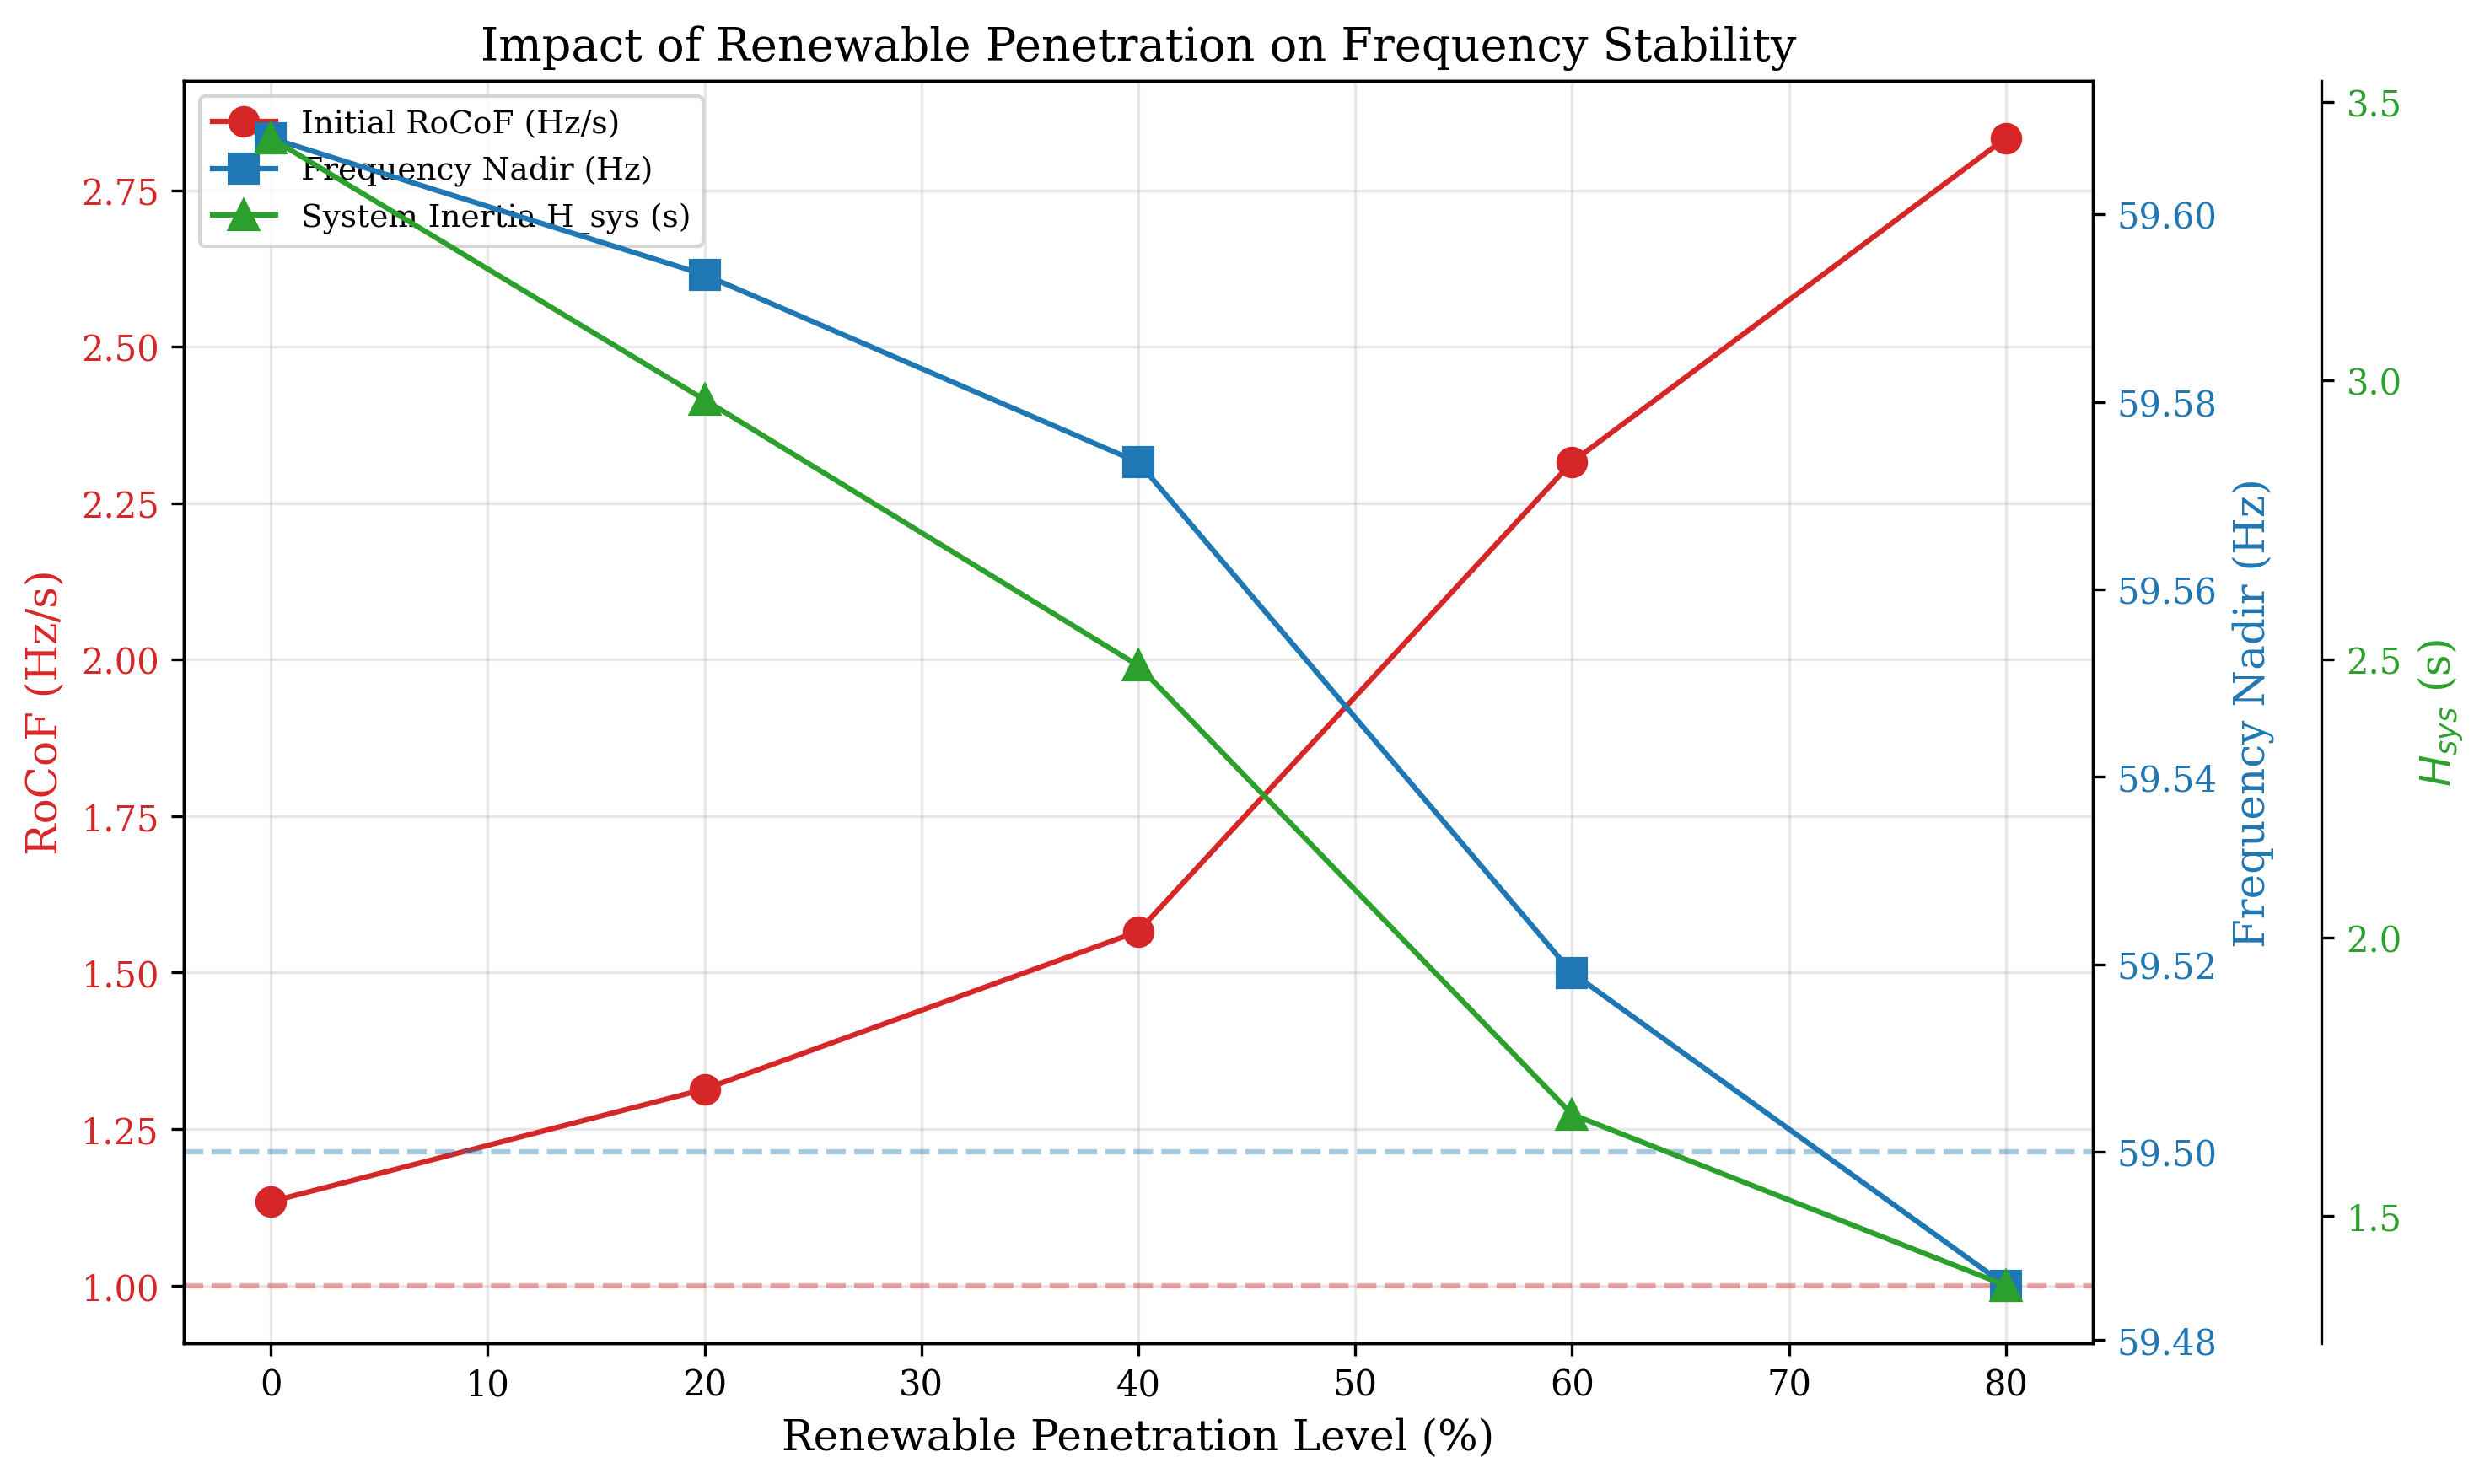
\includegraphics[width=\columnwidth]{fig3_penetration_study.png}
\caption{Impact of renewable penetration on RoCoF, frequency nadir, and system inertia $H_{\mathrm{sys}}$. Dashed lines indicate grid code limits.}
\label{fig:penetration}
\end{figure}

Several key observations emerge from the results:

\begin{enumerate}
    \item \textbf{Inertia degradation:} $H_{\mathrm{sys}}$ decreases monotonically from 3.436~s at 0\% to 1.375~s at 80\% penetration---a 60\% reduction. The total kinetic energy drops correspondingly from 26{,}454~MWs to 10{,}588~MWs.

    \item \textbf{RoCoF worsening:} The initial RoCoF magnitude increases from 1.134~Hz/s to 2.833~Hz/s---a 2.5$\times$ degradation. The relationship follows the inverse proportionality to $E_{\mathrm{kin}}$ predicted by~(\ref{eq:rocof}).

    \item \textbf{Frequency nadir violation:} At 80\% penetration, the frequency nadir drops to 59.486~Hz, violating the 59.5~Hz limit. This identifies the critical penetration threshold as lying between 60\% and 80\%.

    \item \textbf{Non-linear degradation:} The transition from 40\% to 60\% produces a disproportionately large increase in RoCoF (from $-1.566$ to $-2.316$~Hz/s) because three generators (G2, G3, G1) are replaced simultaneously, removing 6{,}204~MWs of kinetic energy.
\end{enumerate}

\subsection{Spatial Inertia Distribution Under Renewable Penetration}

Fig.~\ref{fig:topology_pen} shows the network topology with inertia overlay at five penetration levels (0\%, 20\%, 40\%, 60\%, 80\%). A consistent color scale is used across all subplots for direct comparison. Generator buses converted to IBRs are marked with magenta borders.

\begin{figure*}[!t]
\centering
\includegraphics[width=\textwidth]{fig8_topology_penetration.png}
\caption{IEEE 39-bus system topology with bus inertia distribution under increasing renewable penetration (0\%--80\%). Magenta borders indicate IBR-replaced generators. Color scale is consistent across all subplots.}
\label{fig:topology_pen}
\end{figure*}

The spatial visualization reveals how inertia weakness propagates through the network as generators are replaced:
\begin{itemize}
    \item At 0\% penetration, inertia is distributed relatively uniformly, with the exception of the periphery near small generators.
    \item At 40\%, with four generators replaced (G8, G5, G7, G4), large regions in the southern portion of the network transition from green to yellow, indicating reduced inertia support.
    \item At 80\%, nearly the entire network appears red except for the immediate vicinity of Bus~38 (G9) and Bus~39 (G10), the only remaining synchronous generators. The concentration of all inertia support in two locations creates a spatially fragile system.
\end{itemize}

Fig.~\ref{fig:inertia_comparison} provides a quantitative comparison of bus-level inertia across penetration scenarios.

\begin{figure}[!t]
\centering
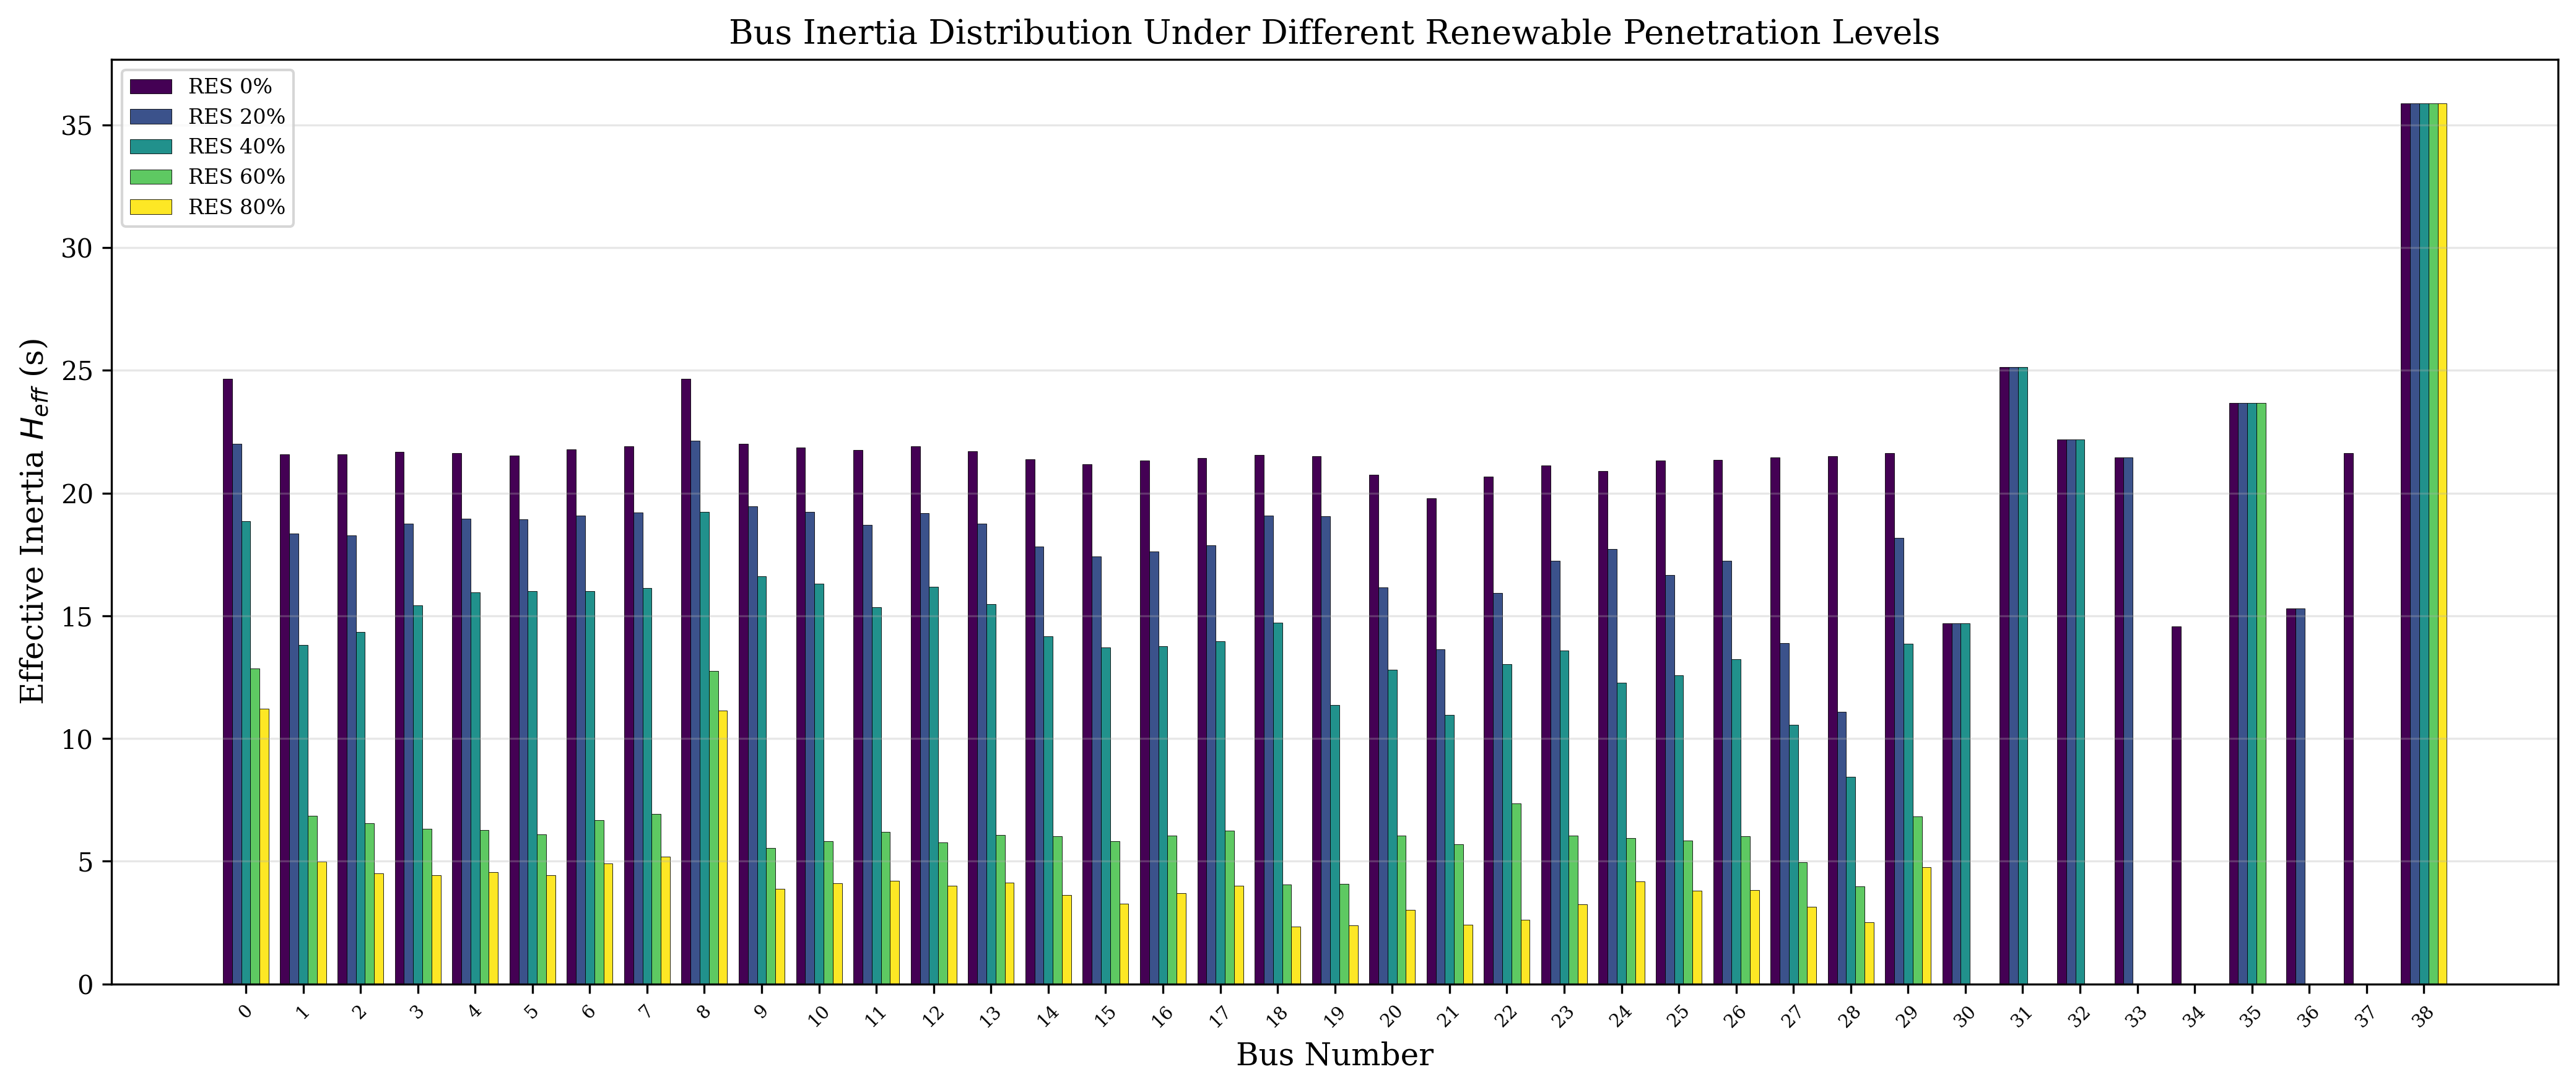
\includegraphics[width=\columnwidth]{fig5_inertia_comparison.png}
\caption{Comparison of effective inertia $H_{\mathrm{eff}}$ at each bus across five renewable penetration scenarios.}
\label{fig:inertia_comparison}
\end{figure}

\subsection{Multi-Machine Frequency Dynamics}

Fig.~\ref{fig:multi_machine} shows the individual generator frequency trajectories and the COI frequency following a G10 trip at 0\% penetration. The heterogeneous response is clearly visible: generators with lower inertia constants (e.g., G5 with $H = 2.60$~s) exhibit faster frequency decline compared to higher-inertia machines (e.g., G9 with $H = 3.45$~s).

\begin{figure}[!t]
\centering
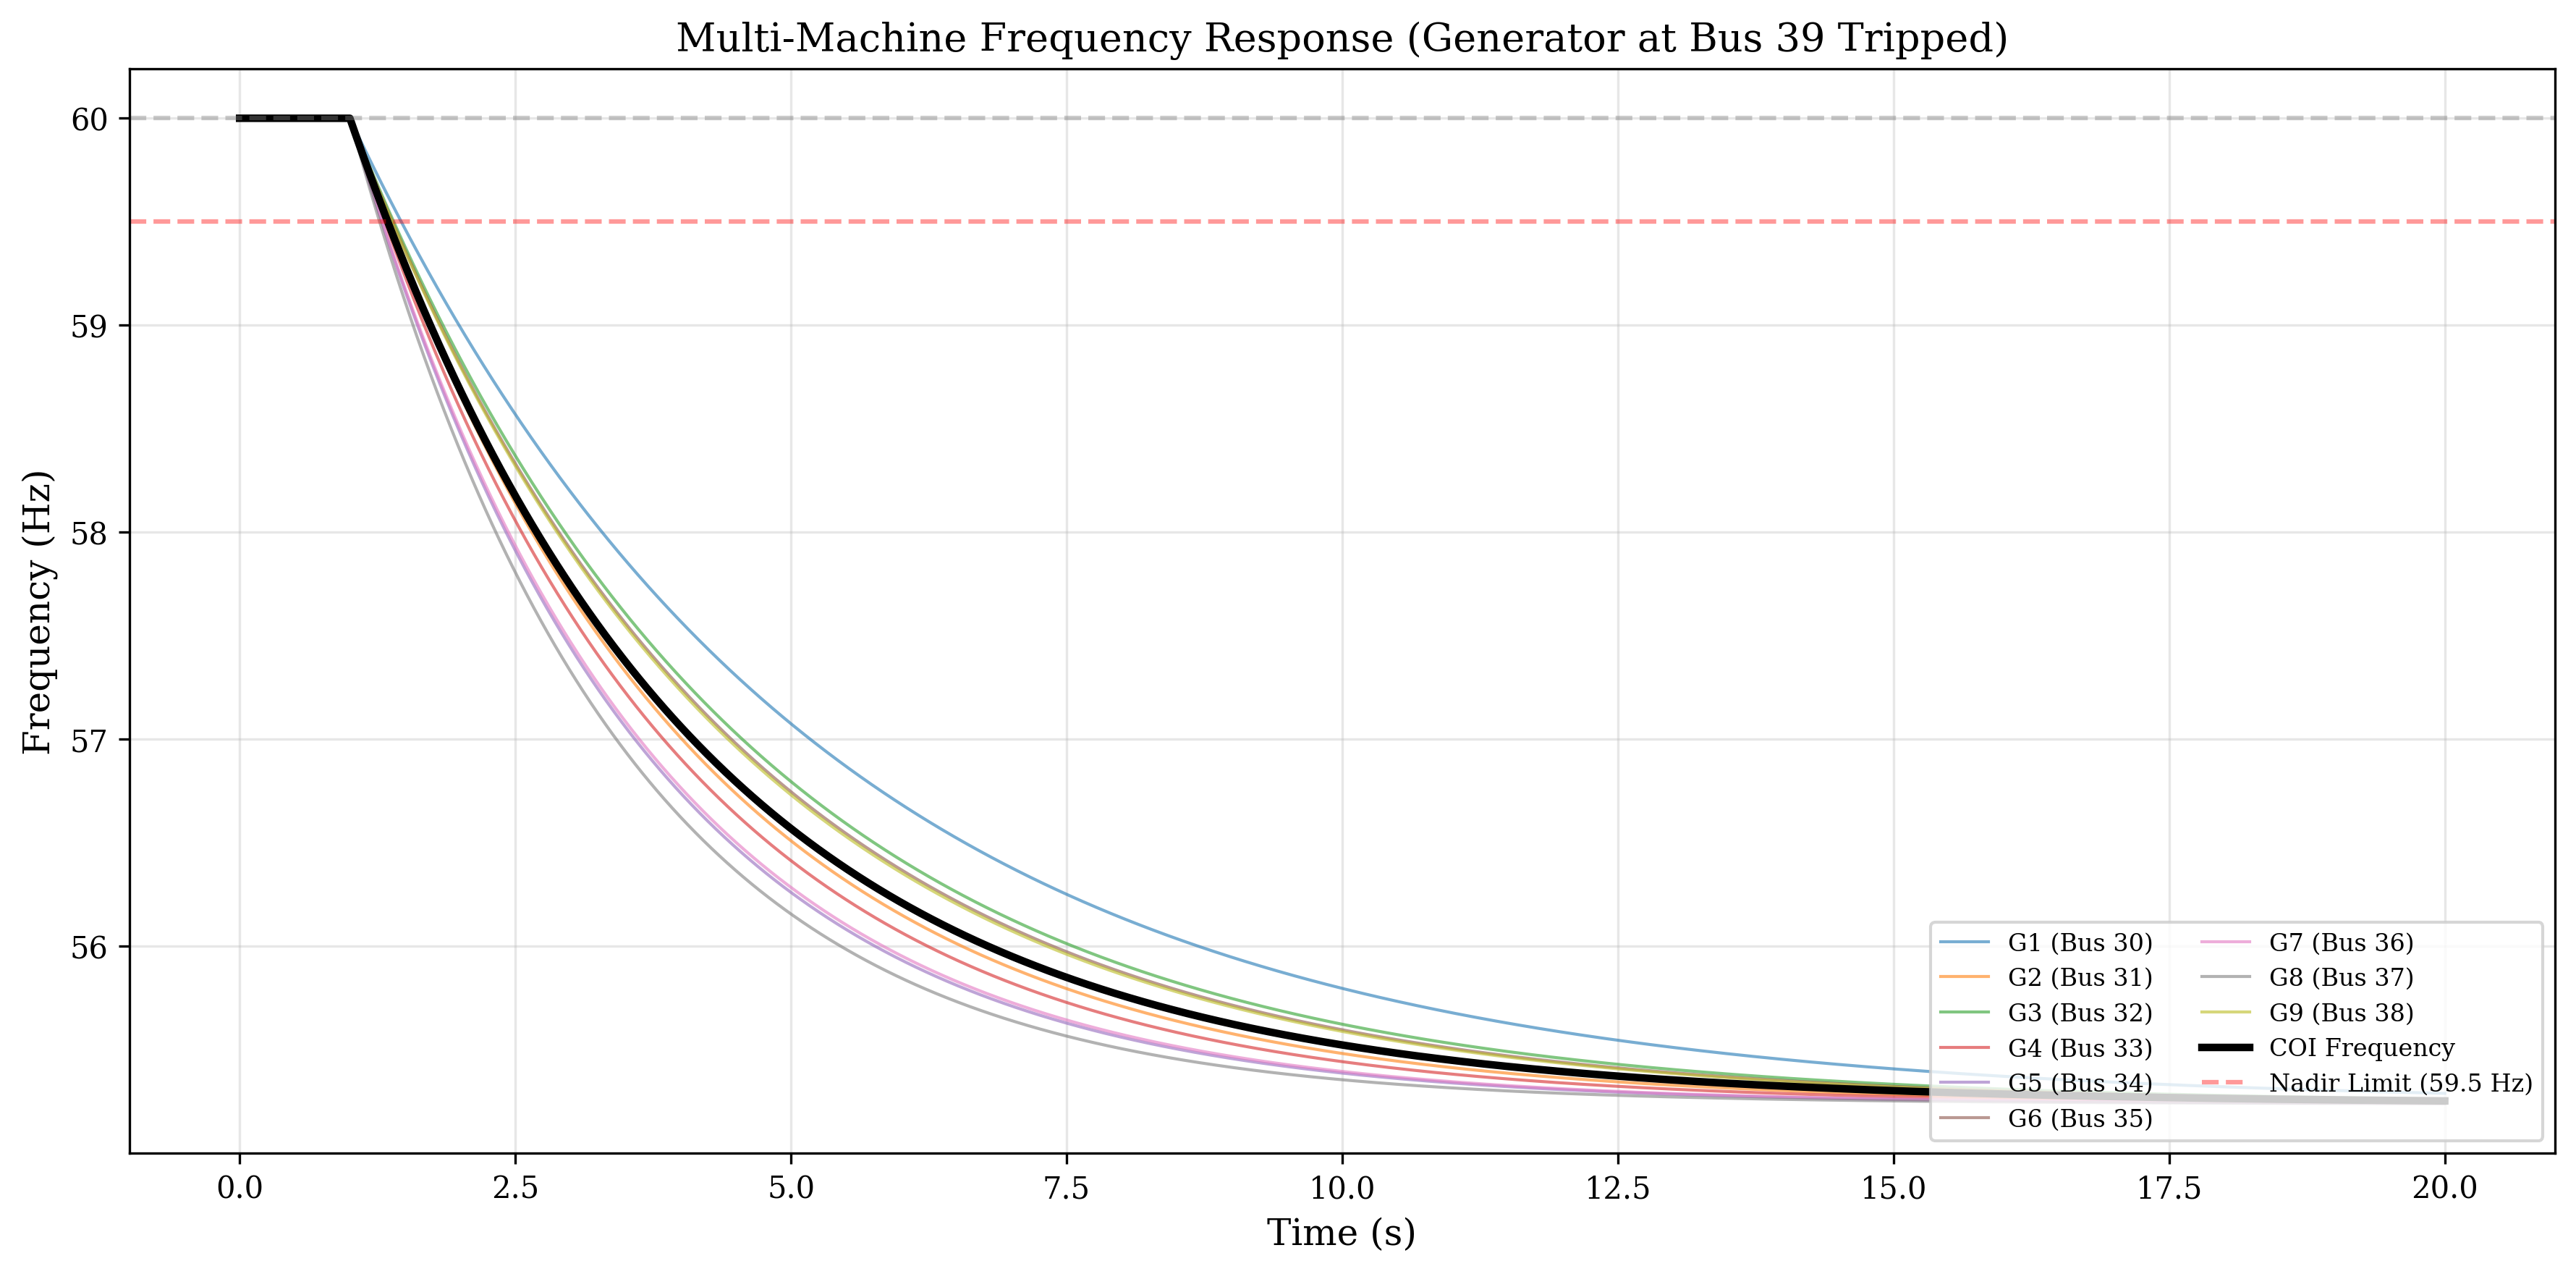
\includegraphics[width=\columnwidth]{fig4_multi_machine_pen0.png}
\caption{Multi-machine frequency response after G10 trip (0\% RES penetration). Individual generator frequencies and COI frequency are shown.}
\label{fig:multi_machine}
\end{figure}

At elevated penetration levels, the frequency dynamics become progressively more severe. With only two synchronous generators remaining at 60\% penetration, the COI frequency nadir drops to 42.63~Hz---far below any acceptable operating threshold---demonstrating the fundamental instability of systems with insufficient inertia.

% ============================================================================
\section{Conclusion}
\label{sec:conclusion}
% ============================================================================

This paper presented a comprehensive bus-level inertia distribution analysis on the IEEE 39-bus New England system under increasing renewable energy penetration. The key findings are summarized as follows:

\begin{enumerate}
    \item The effective inertia varies significantly across buses, with a 2.5:1 ratio between the highest (Bus~38, $H_{\mathrm{eff}} = 35.88$~s) and lowest (Bus~34, $H_{\mathrm{eff}} = 14.56$~s) buses, demonstrating the spatial heterogeneity of inertia support.

    \item Ten inertia-weak buses were identified, clustering in two regions: the southern network area (Buses~20--24) and generator buses with small-rated machines (G1, G5, G7).

    \item The critical renewable penetration threshold lies between 60\% and 80\%, beyond which the frequency nadir violates the 59.5~Hz grid code limit for the worst-case generator trip scenario (G10, 1{,}000~MW).

    \item At 80\% penetration, system inertia is reduced by 60\% and RoCoF worsens by a factor of 2.5, with inertia support concentrated in only two generator locations.

    \item The network topology visualization with inertia overlay provides an effective tool for identifying spatially vulnerable regions requiring virtual inertia support.
\end{enumerate}

Future work will incorporate virtual inertia placement optimization at inertia-weak buses, battery energy storage system (BESS) sizing for synthetic inertia provision, and validation on larger test systems with realistic renewable generation profiles.

% ============================================================================
% References
% ============================================================================

\begin{thebibliography}{99}

\bibitem{kundur1994}
P.~Kundur, \textit{Power System Stability and Control}. New York, NY, USA: McGraw-Hill, 1994.

\bibitem{ulbig2014}
A.~Ulbig, T.~S.~Borsche, and G.~Andersson, ``Impact of low rotational inertia on power system stability and operation,'' \textit{IFAC Proc. Volumes}, vol.~47, no.~3, pp.~7290--7297, 2014.

\bibitem{milano2018}
F.~Milano, F.~D\"{o}rfler, G.~Hug, D.~J.~Hill, and G.~Verbi\v{c}, ``Foundations and challenges of low-inertia systems,'' in \textit{Proc. 20th Power Syst. Comput. Conf. (PSCC)}, Dublin, Ireland, Jun. 2018, pp.~37--61.

\bibitem{bevrani2014}
H.~Bevrani, T.~Ise, and Y.~Miura, ``Virtual synchronous generators: A survey and new perspectives,'' \textit{Int. J. Electr. Power Energy Syst.}, vol.~54, pp.~244--254, Jan. 2014.

\bibitem{fernandez2019}
A.~Fern\'{a}ndez-Guillam\'{o}n, E.~G\'{o}mez-L\'{a}zaro, E.~Muljadi, and \'{A}.~Molina-Garc\'{i}a, ``Power systems with high renewable energy sources: A review of inertia and frequency control strategies over time,'' \textit{Renew. Sustain. Energy Rev.}, vol.~115, Art.~no.~109369, Nov. 2019.

\bibitem{dreidy2017}
M.~Dreidy, H.~Mokhlis, and S.~Mekhilef, ``Inertia response and frequency control techniques for renewable energy sources: A review,'' \textit{Renew. Sustain. Energy Rev.}, vol.~69, pp.~144--155, Mar. 2017.

\bibitem{tuo2021}
M.~Tuo and X.~Li, ``Dynamic estimation of power system inertia distribution using synchrophasor measurements,'' in \textit{Proc. IEEE North Amer. Power Symp. (NAPS)}, Nov. 2021, pp.~1--6.

\bibitem{li2024}
Z.~Li, W.~Ye, \textit{et al.}, ``New energy power system inertia weak position evaluation and frequency monitoring positioning,'' \textit{Frontiers Energy Res.}, vol.~12, Art.~no.~1418302, 2024.

\end{thebibliography}

\begin{IEEEbiography}[{\includegraphics[width=1in,height=1.25in,clip,keepaspectratio]{}}]{Shakil}
received the B.Eng. degree. He is currently pursuing the M.Eng. degree with the Department of Electrical and Electronic Engineering, University of Fukui, Fukui, Japan. His research interests include power system stability, renewable energy integration, and frequency control.
\end{IEEEbiography}

\begin{IEEEbiography}[{\includegraphics[width=1in,height=1.25in,clip,keepaspectratio]{}}]{Ryuto Shigenobu}
(Member, IEEE) received the Ph.D. degree. He is currently with the Department of Electrical and Electronic Engineering, University of Fukui, Fukui, Japan. His research interests include power system analysis, smart grids, and distributed energy resources.
\end{IEEEbiography}

\end{document}
